\documentclass[]{article}
\title{Lab 4\\GPIO}
\author{Keaton Clark\\Partner: Abigail Dolan}
\usepackage{graphicx}
\usepackage{listings}
\usepackage{xcolor}
\begin{document}
\maketitle
\definecolor{codegreen}{HTML}{859900}
\definecolor{codegray}{HTML}{839496}
\definecolor{codepurple}{HTML}{6C71C4}
\definecolor{codemagenta}{HTML}{d33682}
\definecolor{backcolour}{HTML}{FDF6E3}
\definecolor{fontcolor}{HTML}{002B36}
\lstdefinestyle{mystyle}{
	basicstyle=\color{fontcolor},
	backgroundcolor=\color{backcolour},   
	commentstyle=\color{codegreen},
	keywordstyle=\color{codemagenta},
	numberstyle=\tiny\color{codegray},
	stringstyle=\color{codepurple},
	breakatwhitespace=false,         
	breaklines=true,                 
	captionpos=b,                    
	keepspaces=true,                 
	numbers=left,                    
	numbersep=5pt,                  
	showspaces=false,                
	showstringspaces=false,
	showtabs=false,                  
	tabsize=4
}
\lstset{style=mystyle}
\section*{Questions}
\subsection*{Part 1}
\begin{enumerate}
	\item The led blinks at approximately 1hz which is the expected frequency given 500ms on and 500ms off.\\
	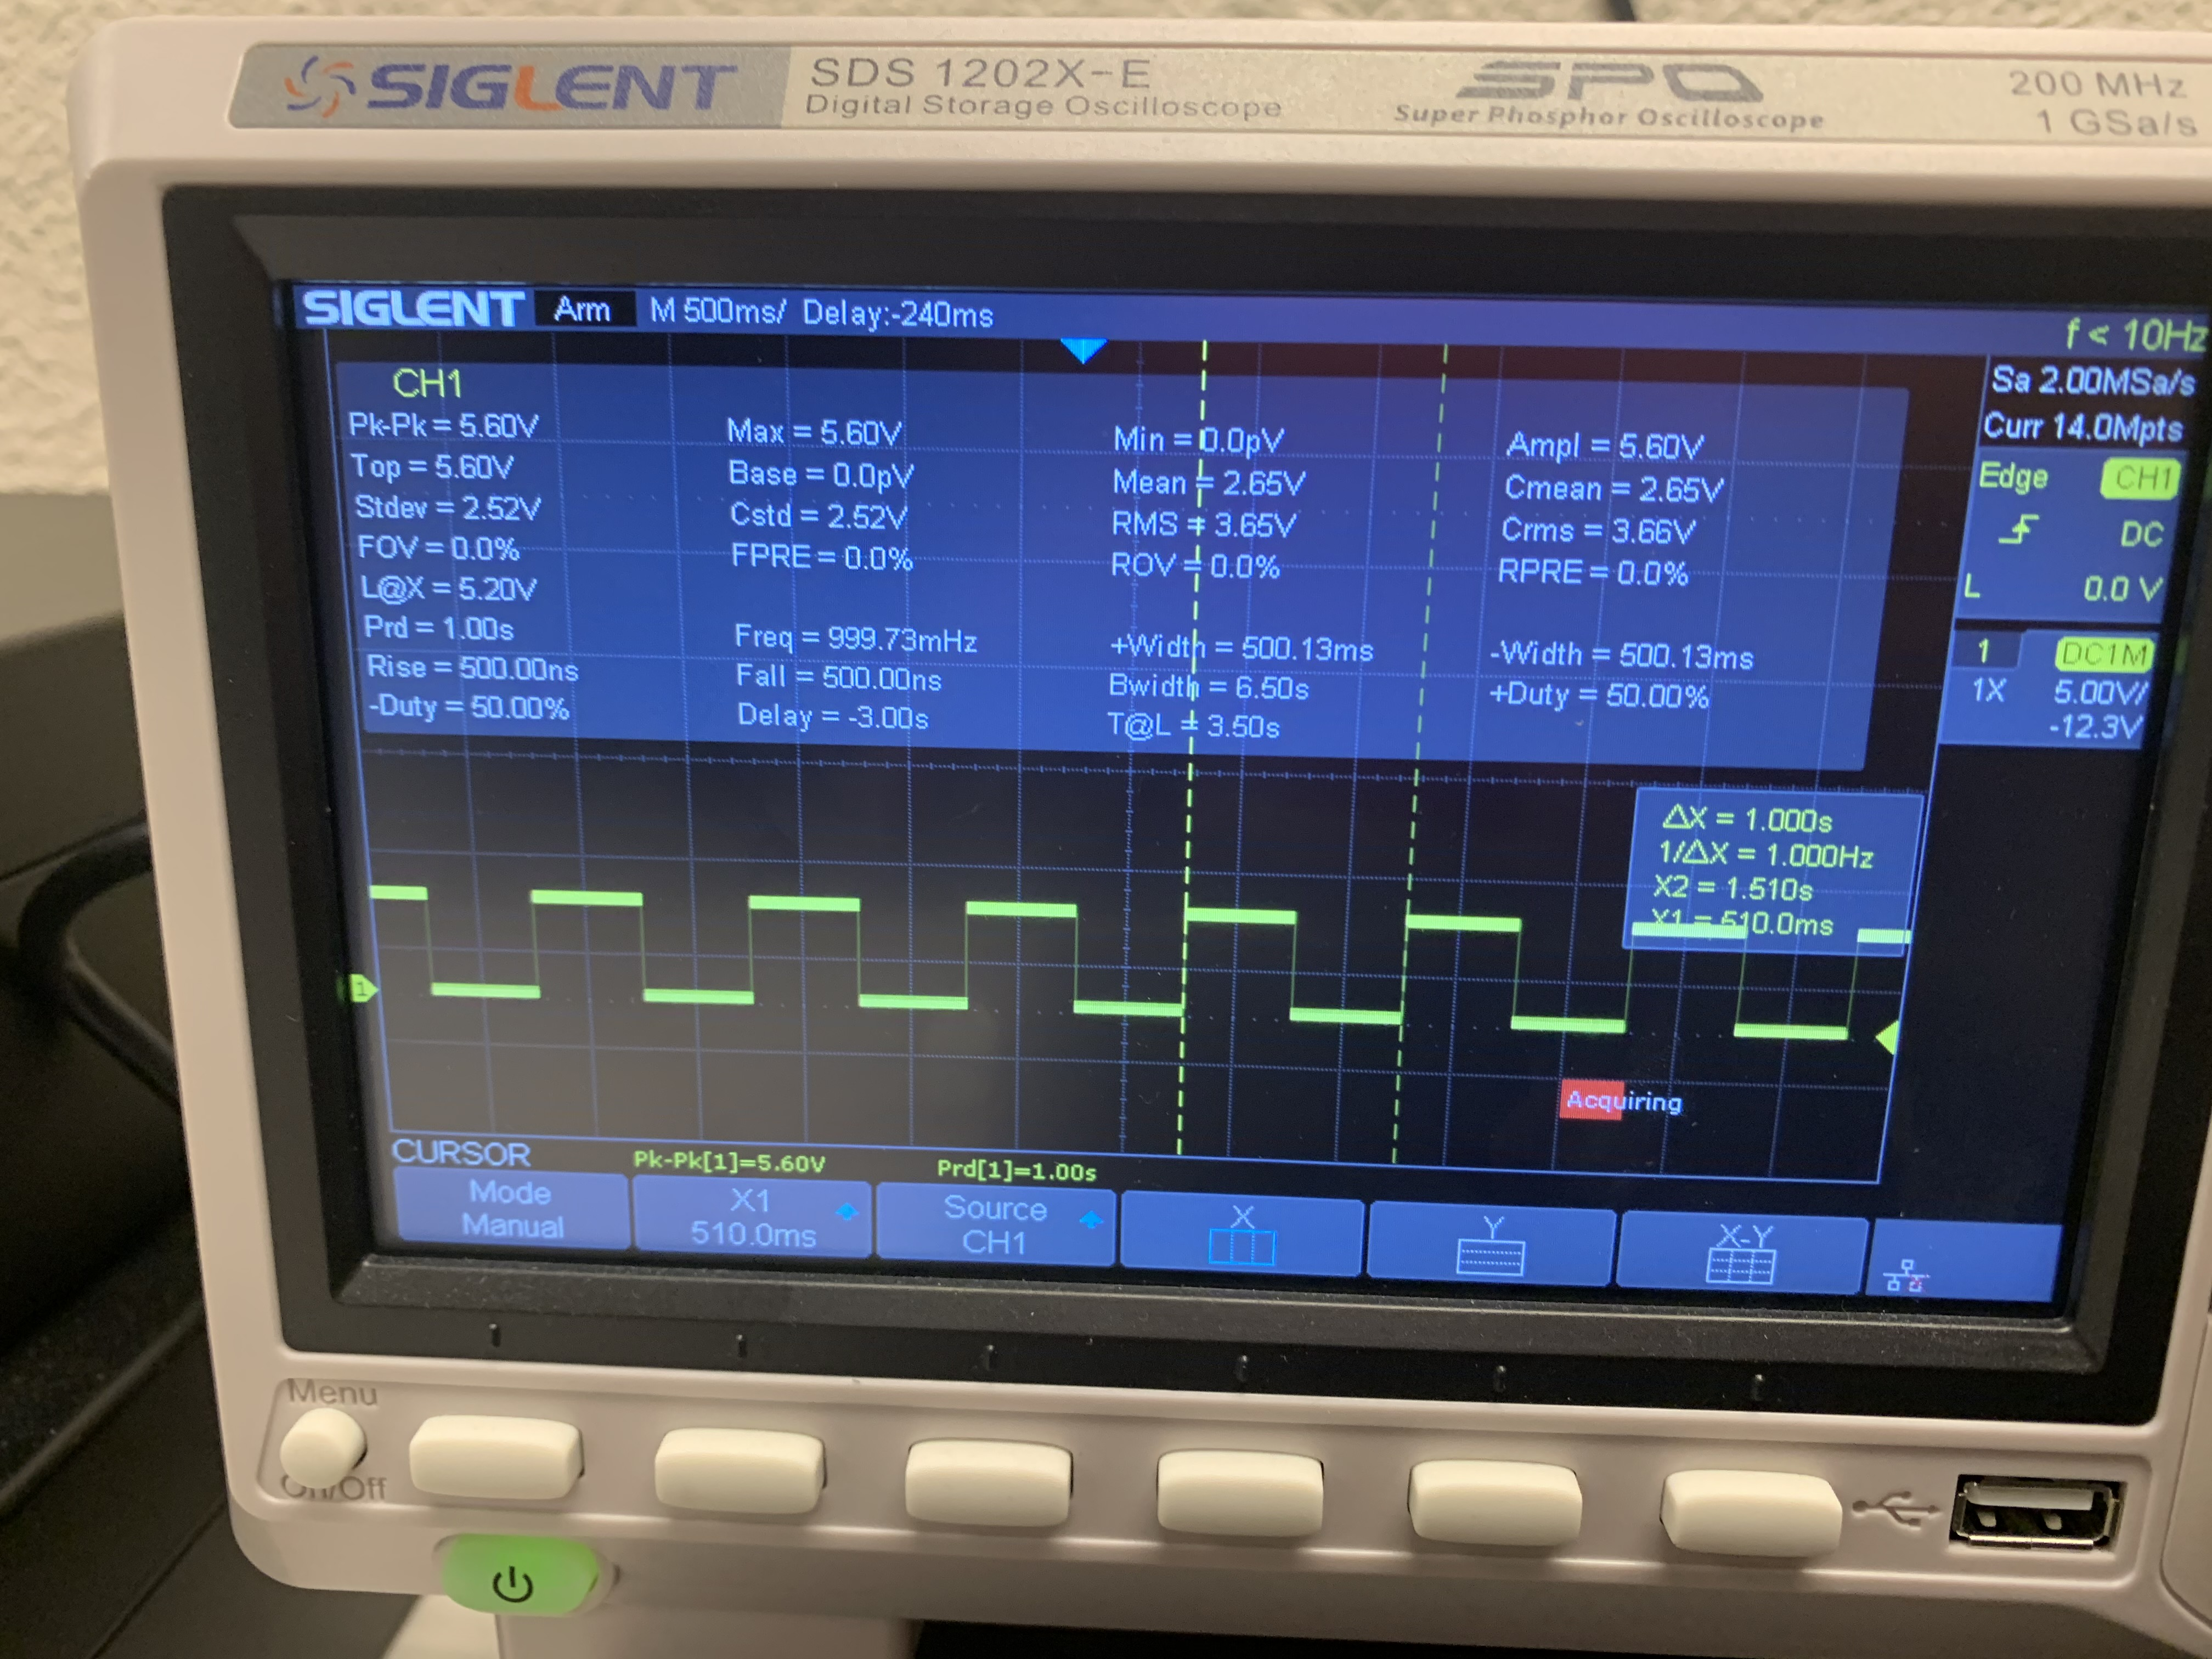
\includegraphics[scale=.1]{images/1-1.jpg}\pagebreak
	\item .5Hz\\
	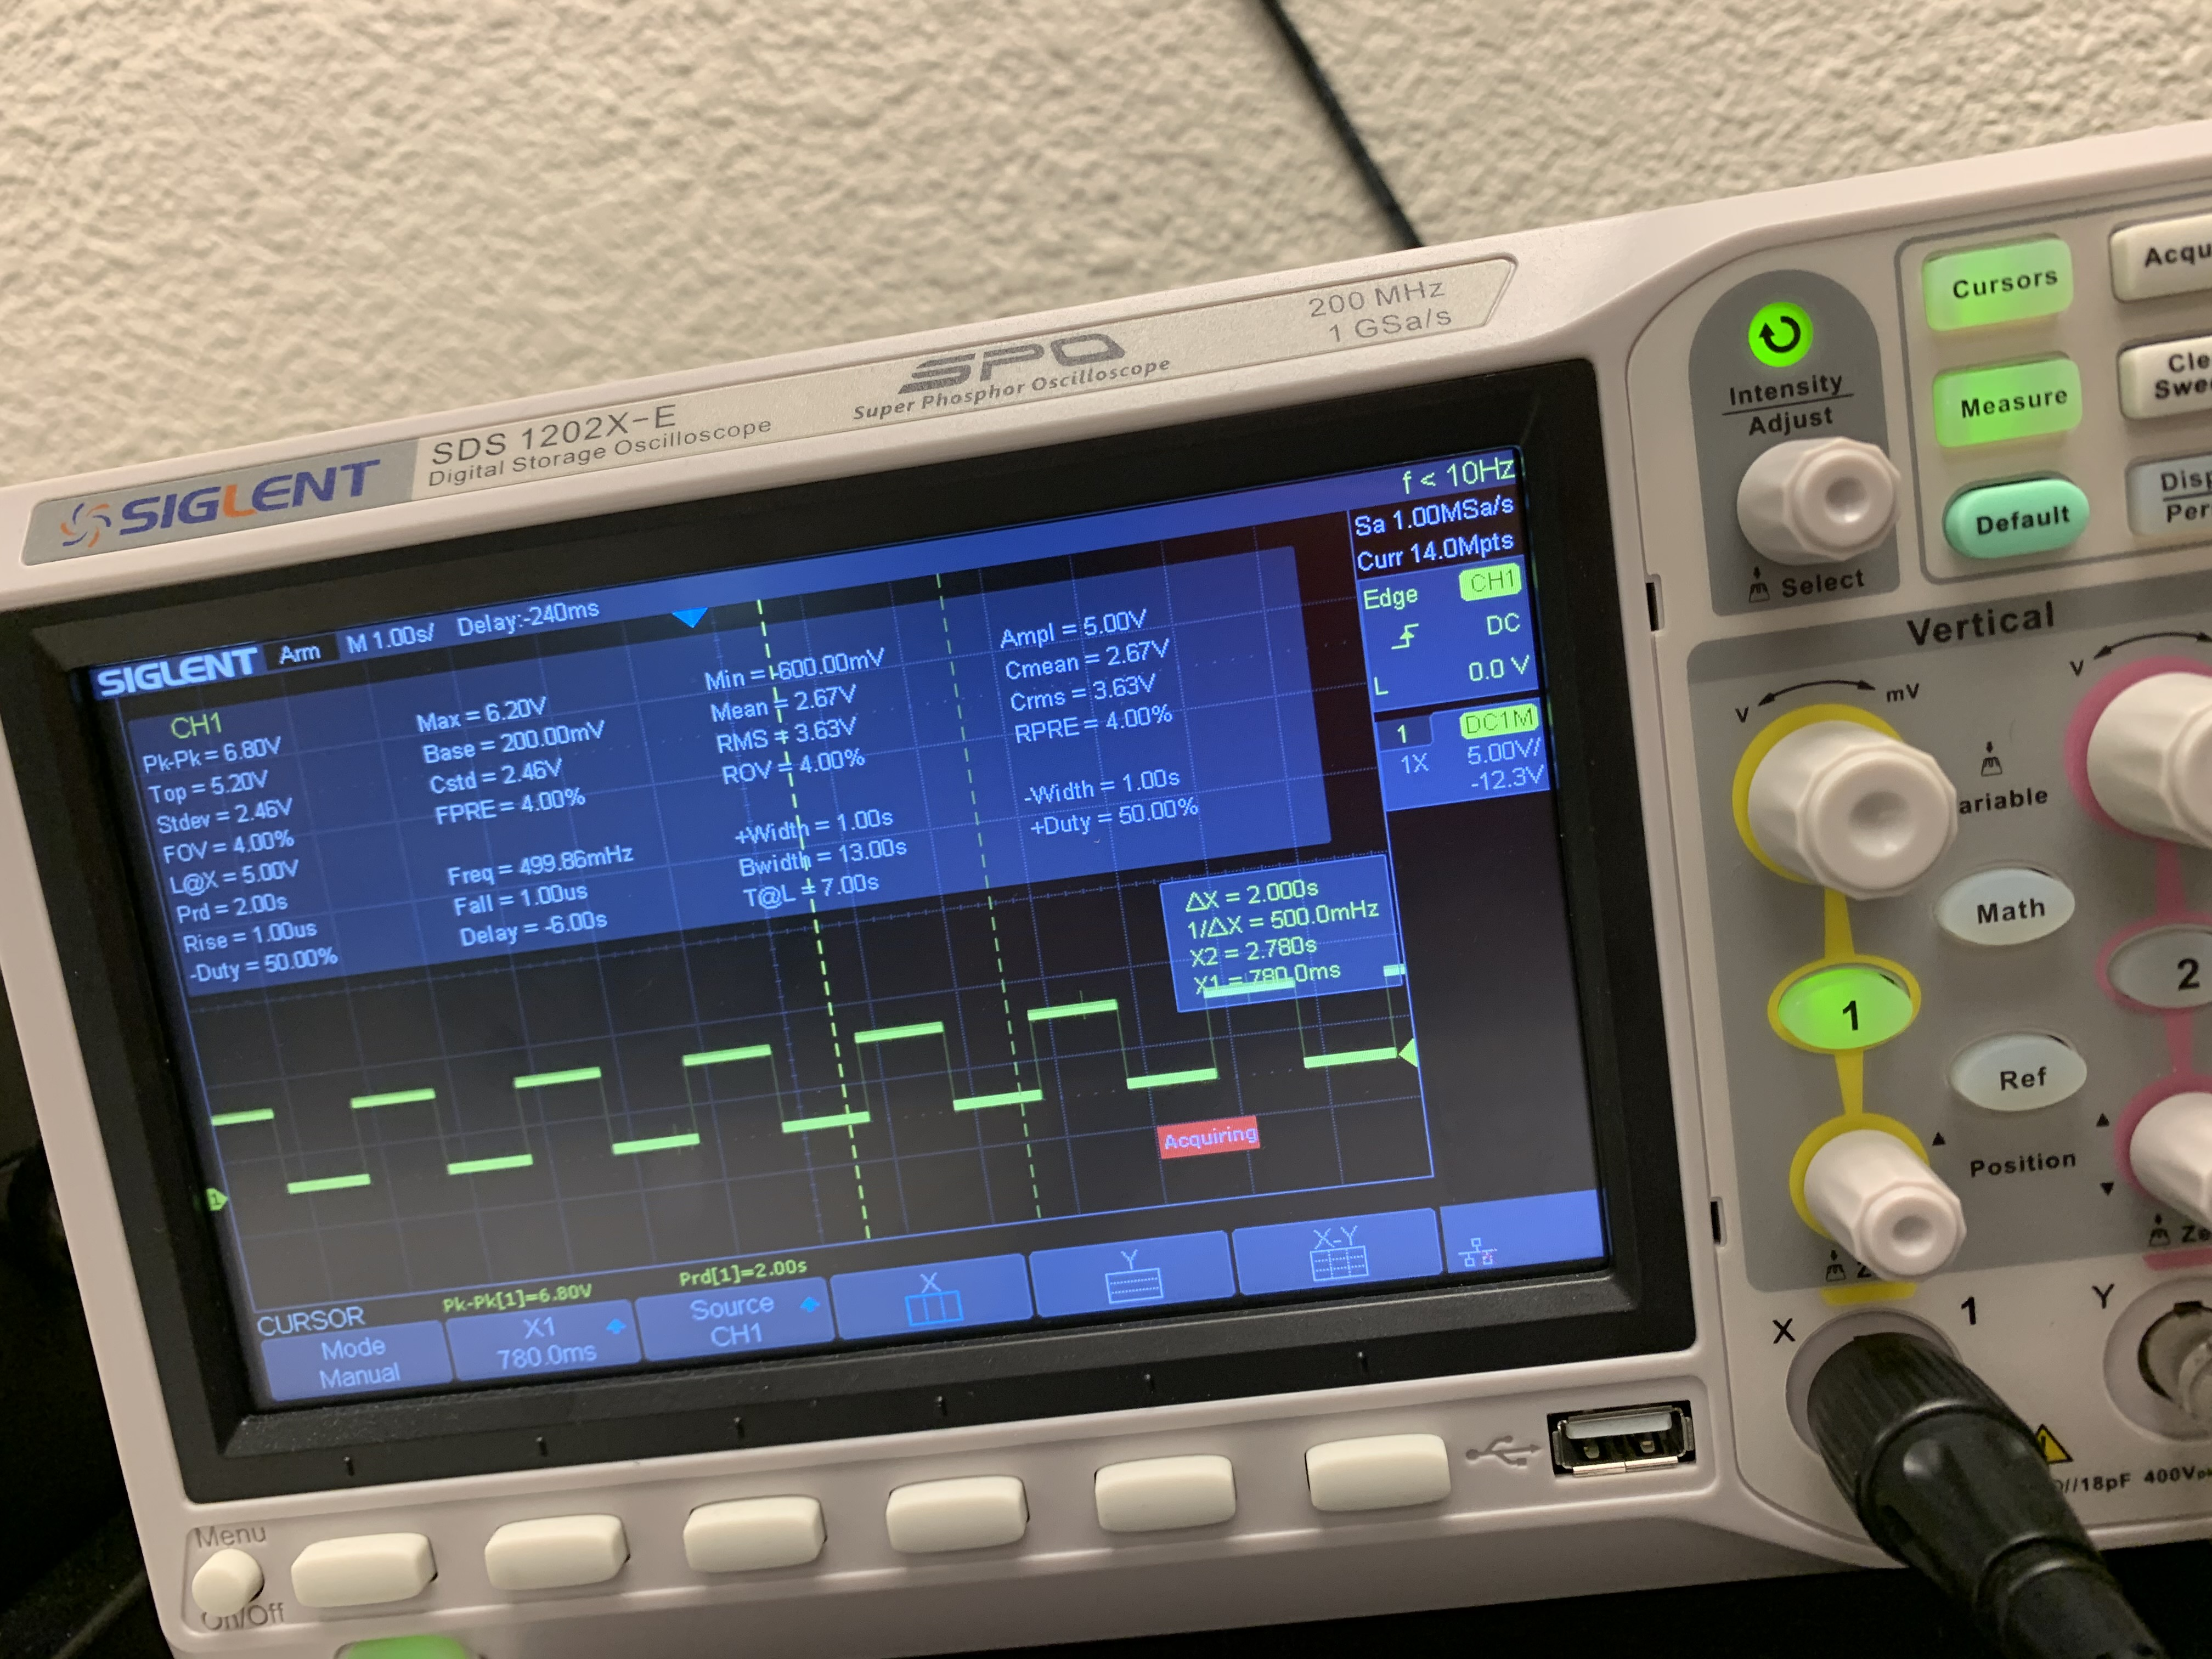
\includegraphics[scale=.1]{images/1-2.jpg}\pagebreak
	\item The frequency after increasing is ~2Hz
	\item With 1ms delay we get 497 Hz\\
	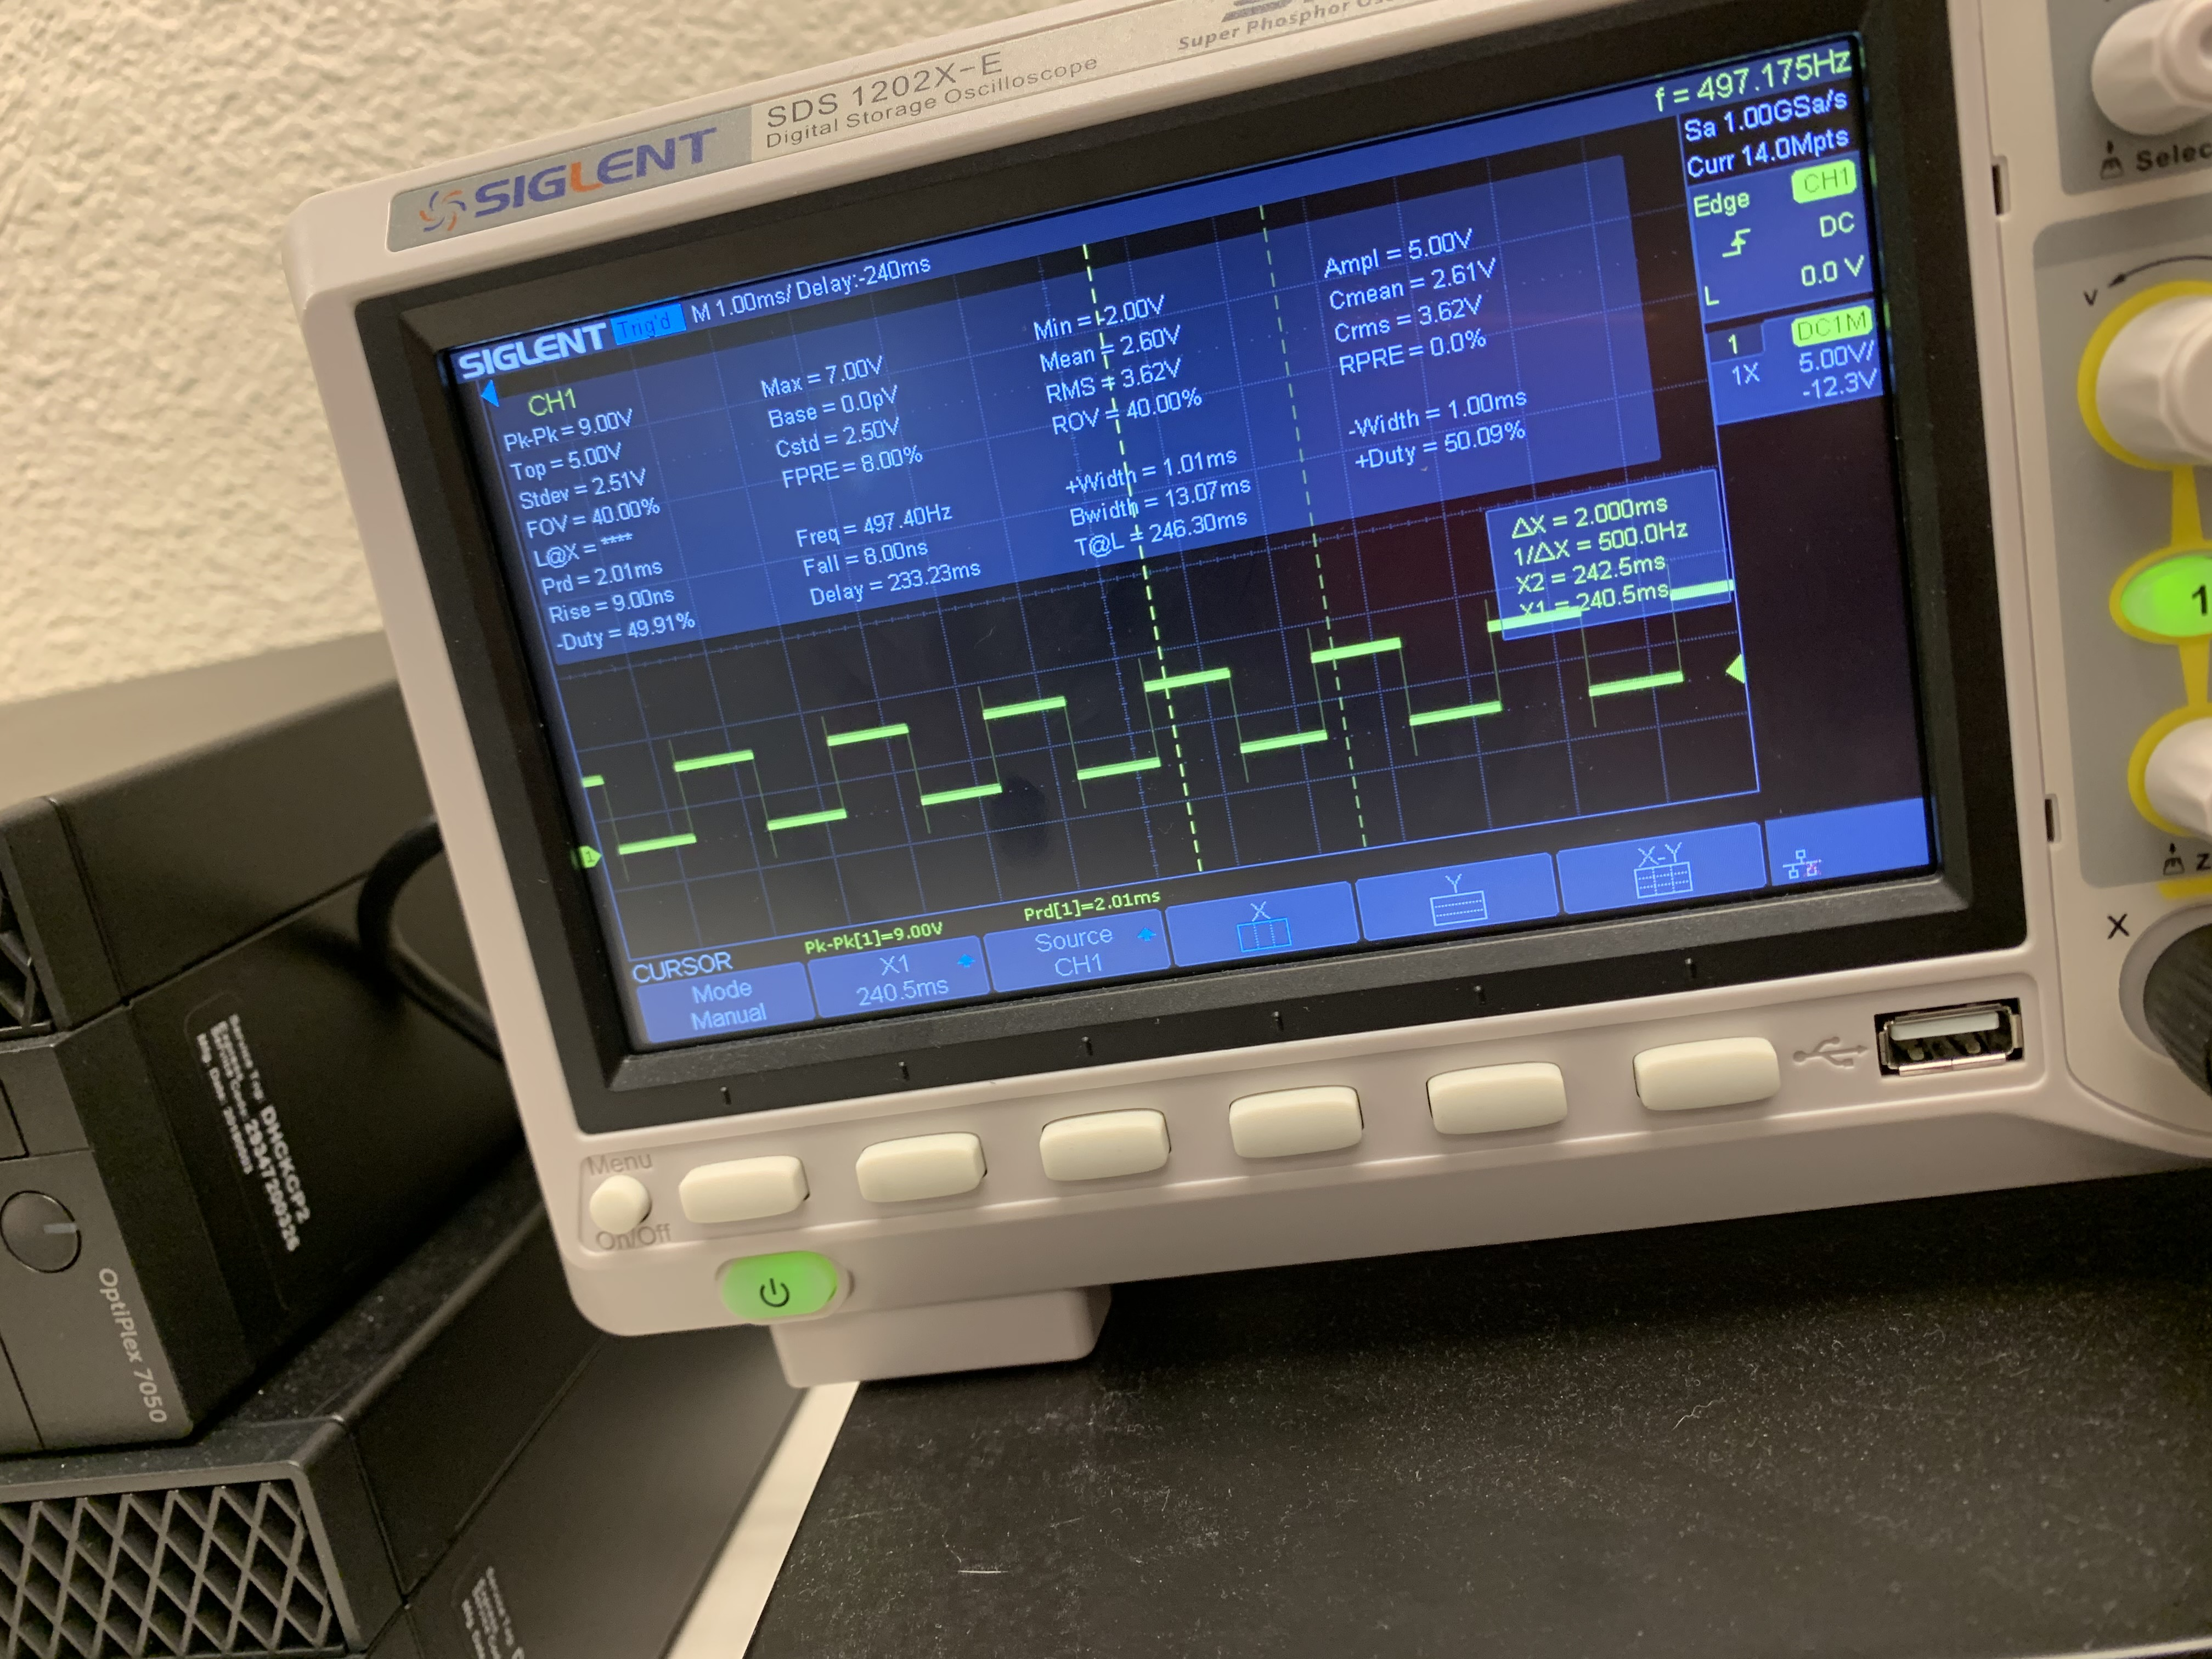
\includegraphics[scale=.1]{images/1-4.jpg}\pagebreak
	\item Done
	\item Active High
	\item Active Low
\end{enumerate}
\subsection*{Part 2}
\begin{enumerate}
	\item 1Hz\\
	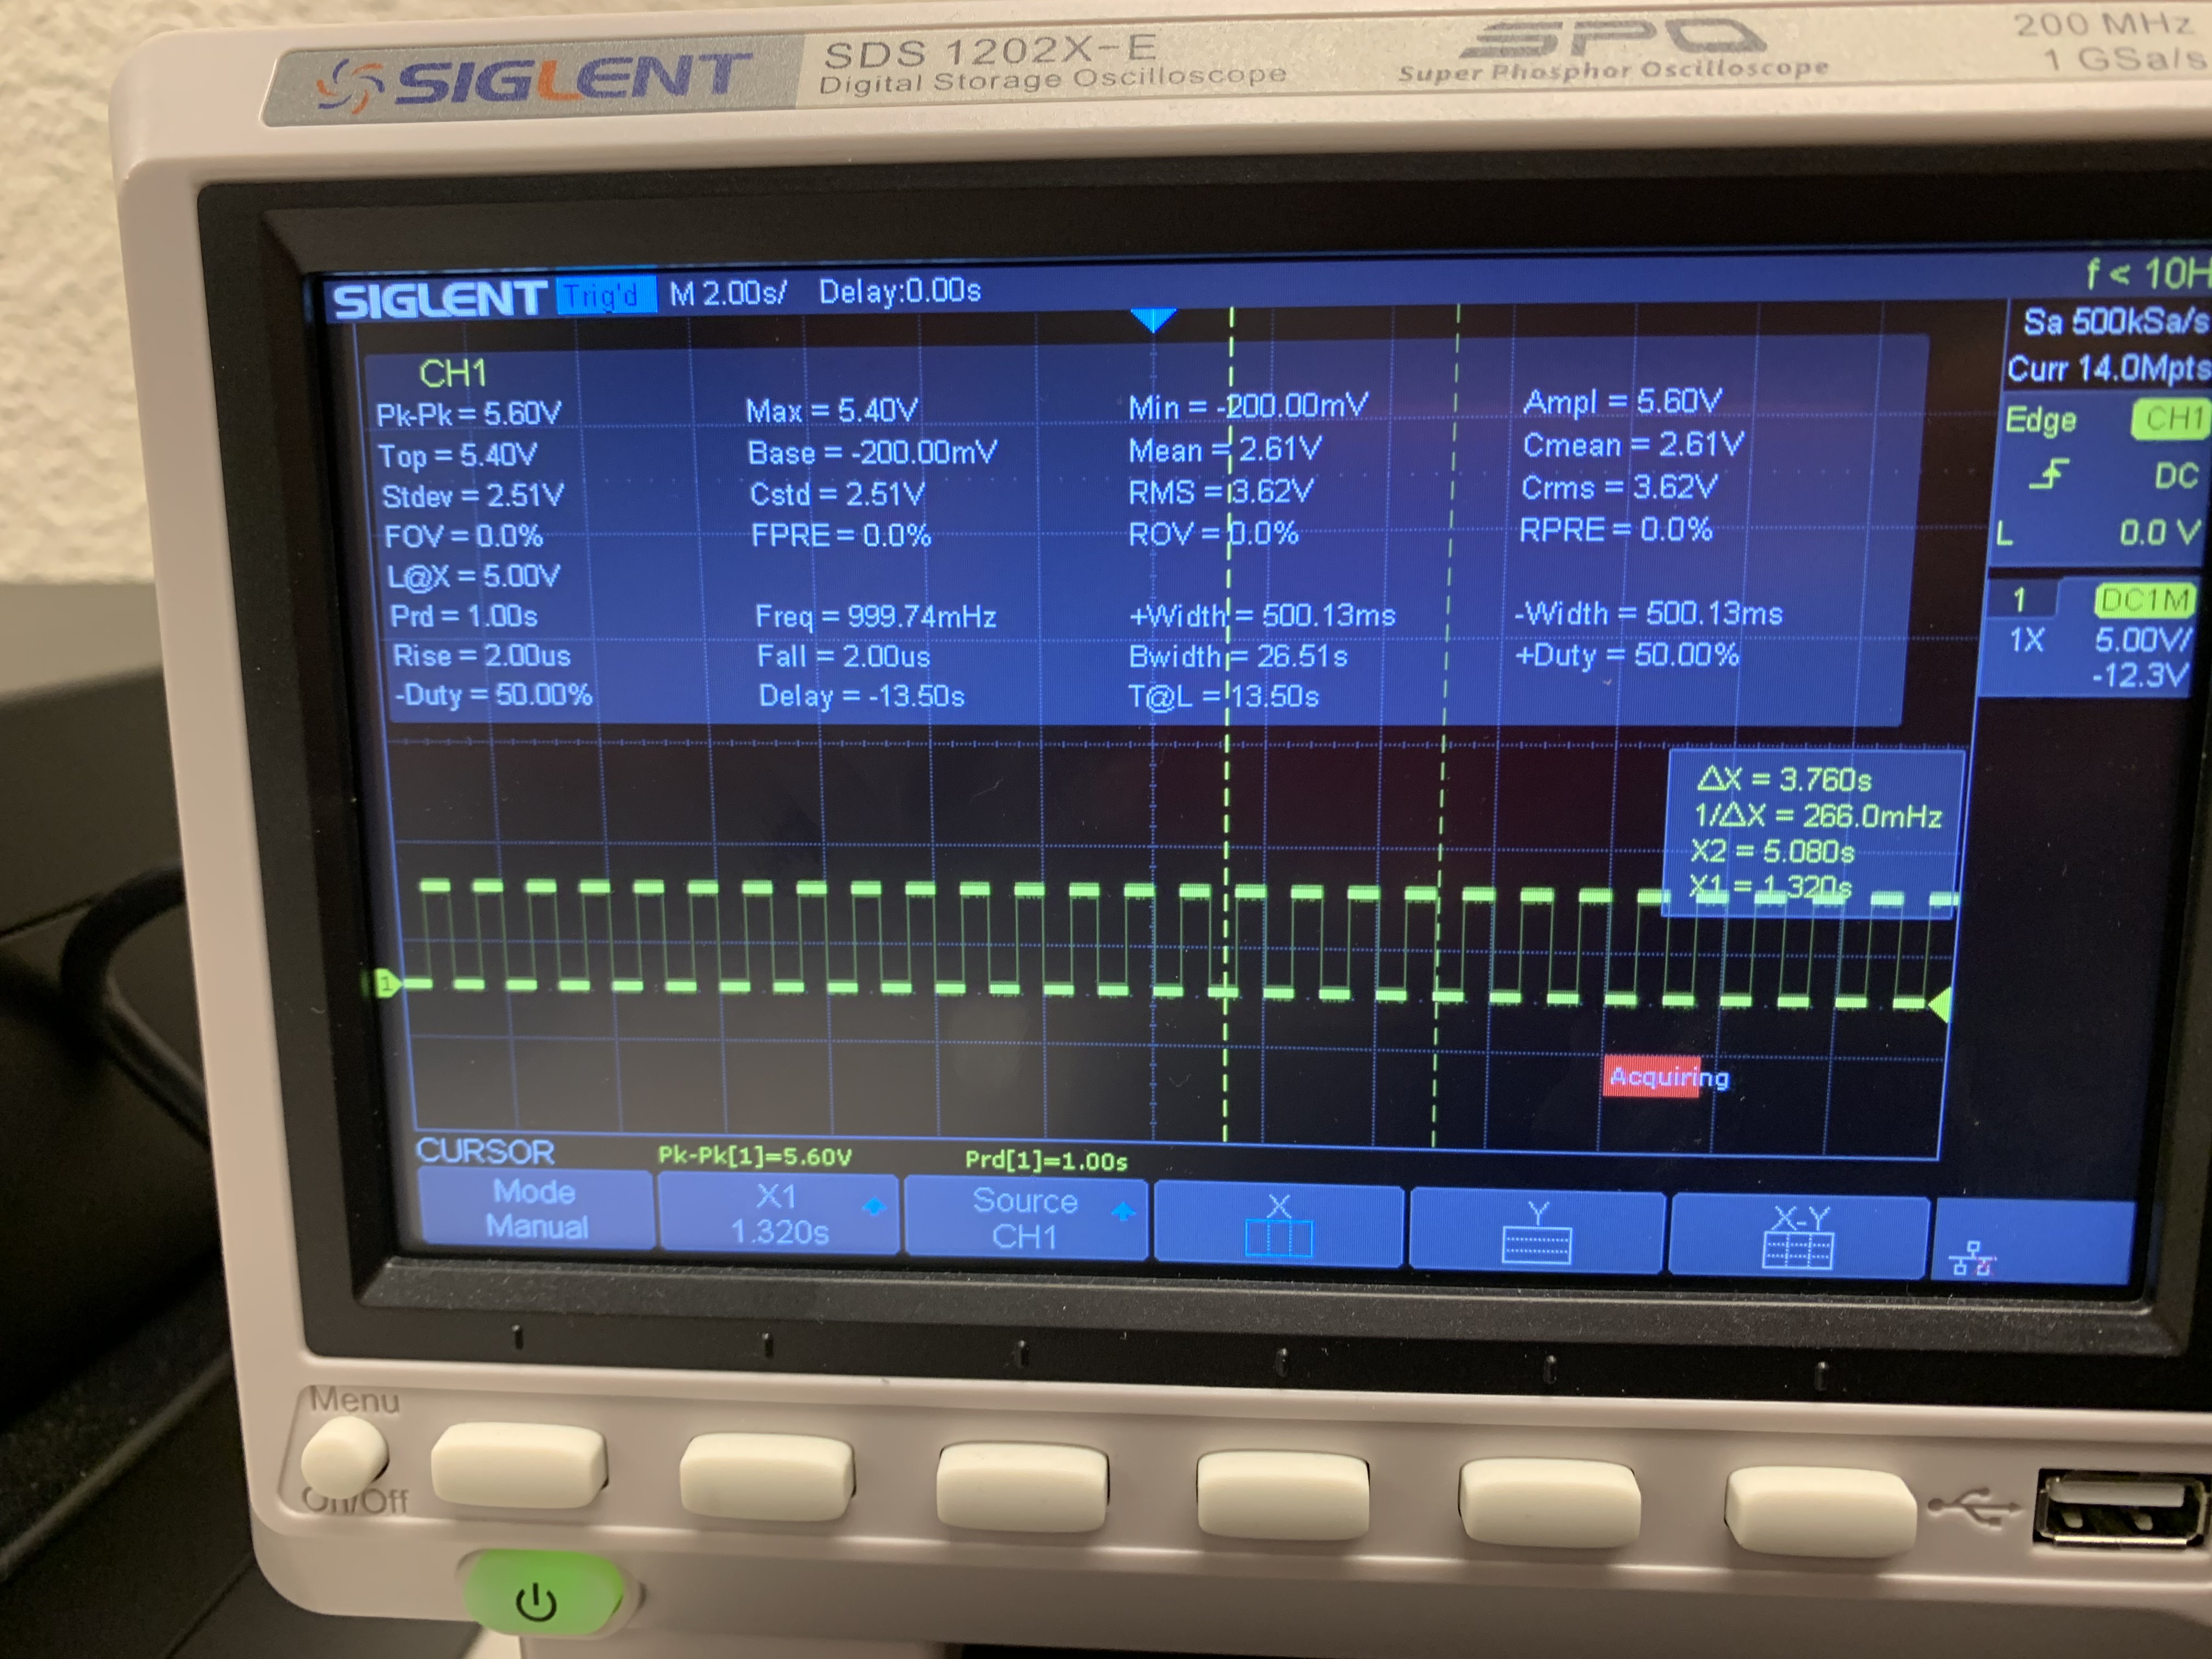
\includegraphics[scale=.1]{images/2-1.jpg}\pagebreak
	\item As fast as possible is no delay. Switching on and off takes 4 operations each to complete so the pulse width is 16,000,000Hz/8 = 2MHz\\
	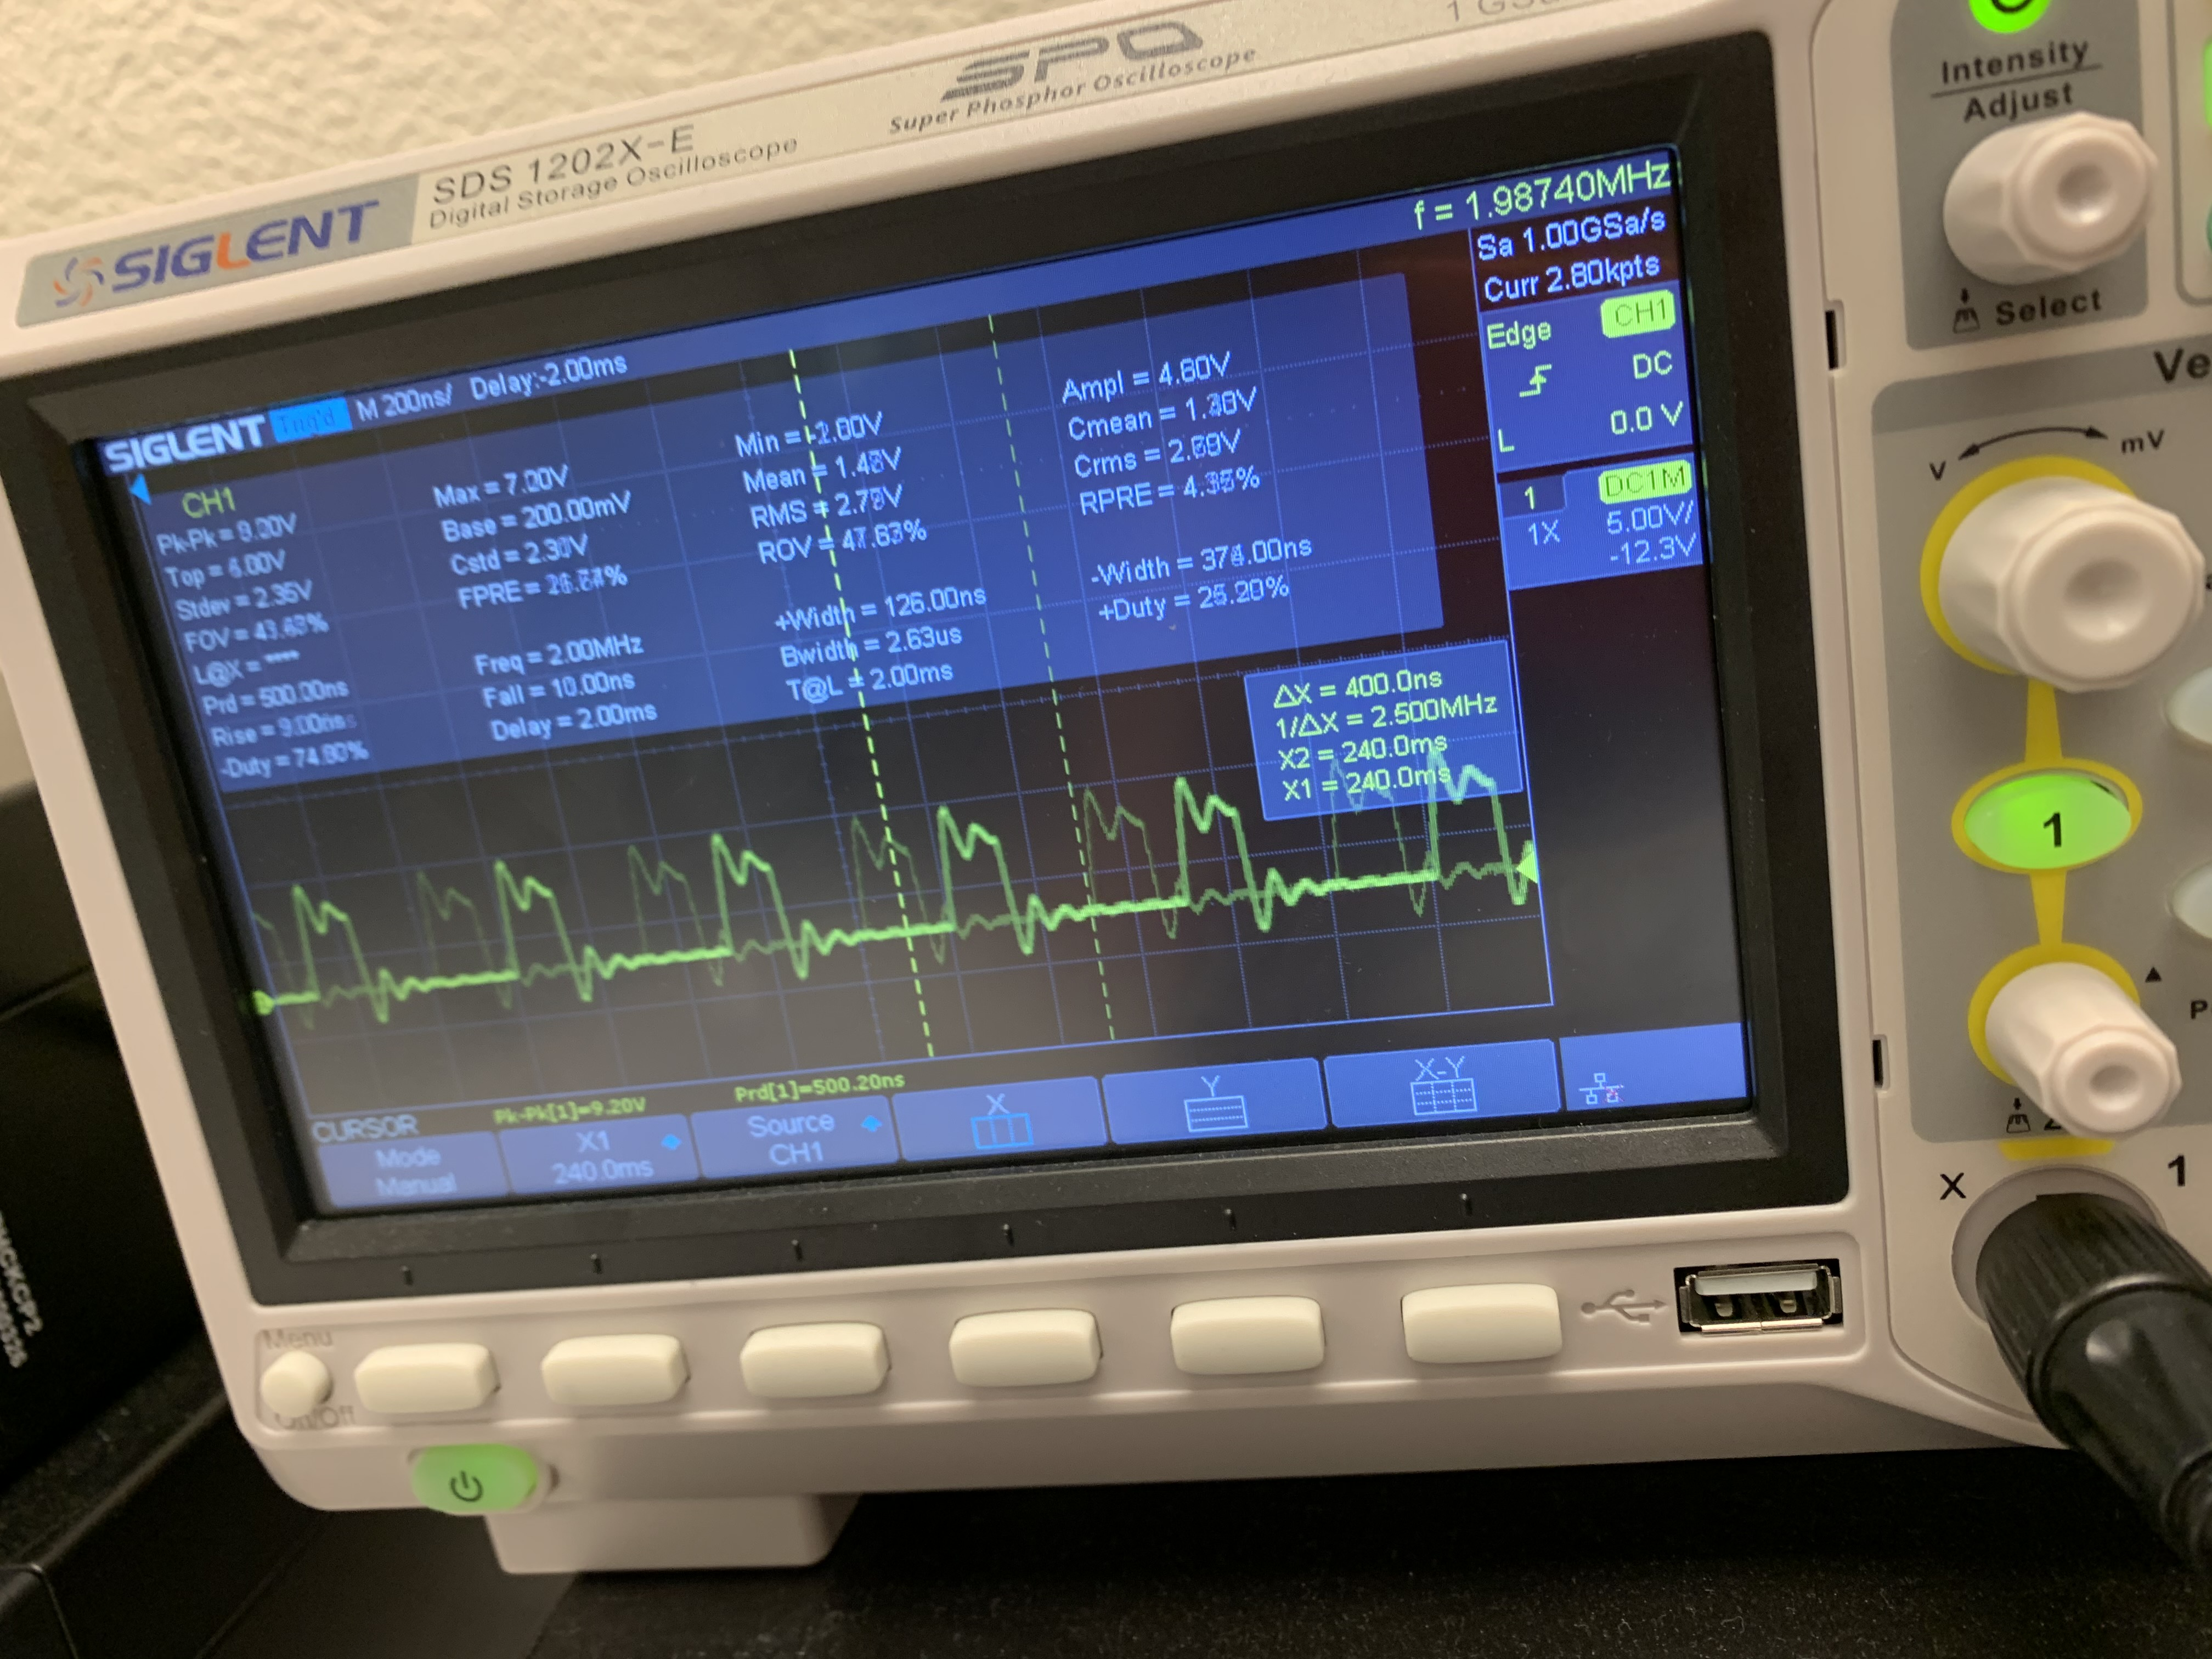
\includegraphics[scale=.1]{images/2-2.jpg}\pagebreak
	\item Total operations it takes to switch the light is what is limiting us. We are at 1/4 of the clock speed.
	\item The functionality of the $|$ symbol is to or the two operands together. The ddr stands for the data direction register and it is an enable to allow the corresponding pin to output.
	\item The or operation returns a 1 in each bit position for which the corresponding bits of either or both operands are 1 and the and operation does the same but both bits in each position must be one. The port or the pin output register tells the microproccessor whether or not to output on that corresponding pin.
\end{enumerate}
\subsection*{Part 3}
\begin{enumerate}
	\item 2 has preprocessor macro functions that expand out to the bit setting and clearing of port b. In 2 he also uses a bit mask instead of the raw hexcode.
	\item 2 has preprocessor macro functions while 3 has actual c functions that are called to set and clear the pins as well as the the data direction register.
	\item
		1=858 bytes\\
		2=858 bytes\\
		3=866 bytes\\
	\item
		1 = 2MHz\\
		2 = 2MHz\\
		3 = 2MHz\\
		We did not percieve any difference with the oscilliscope but we expected 1 and 2 to be the fastest because it should take the fewest operations. This may be down to compiler optimization.
	\item I think that number 2 is the most readable.
\end{enumerate}
\subsection*{Part 4}
\begin{enumerate}
	\item If we did not enable the pullup resistor the input register would be not be stable and would be all over the place and wont be able to read when the button is pressed.
	\item The input is not reliable and doesn't reflect the state of the pin. It is in the third state.
	\item ~250 milliseconds.
\end{enumerate}
\subsection*{Part 5}
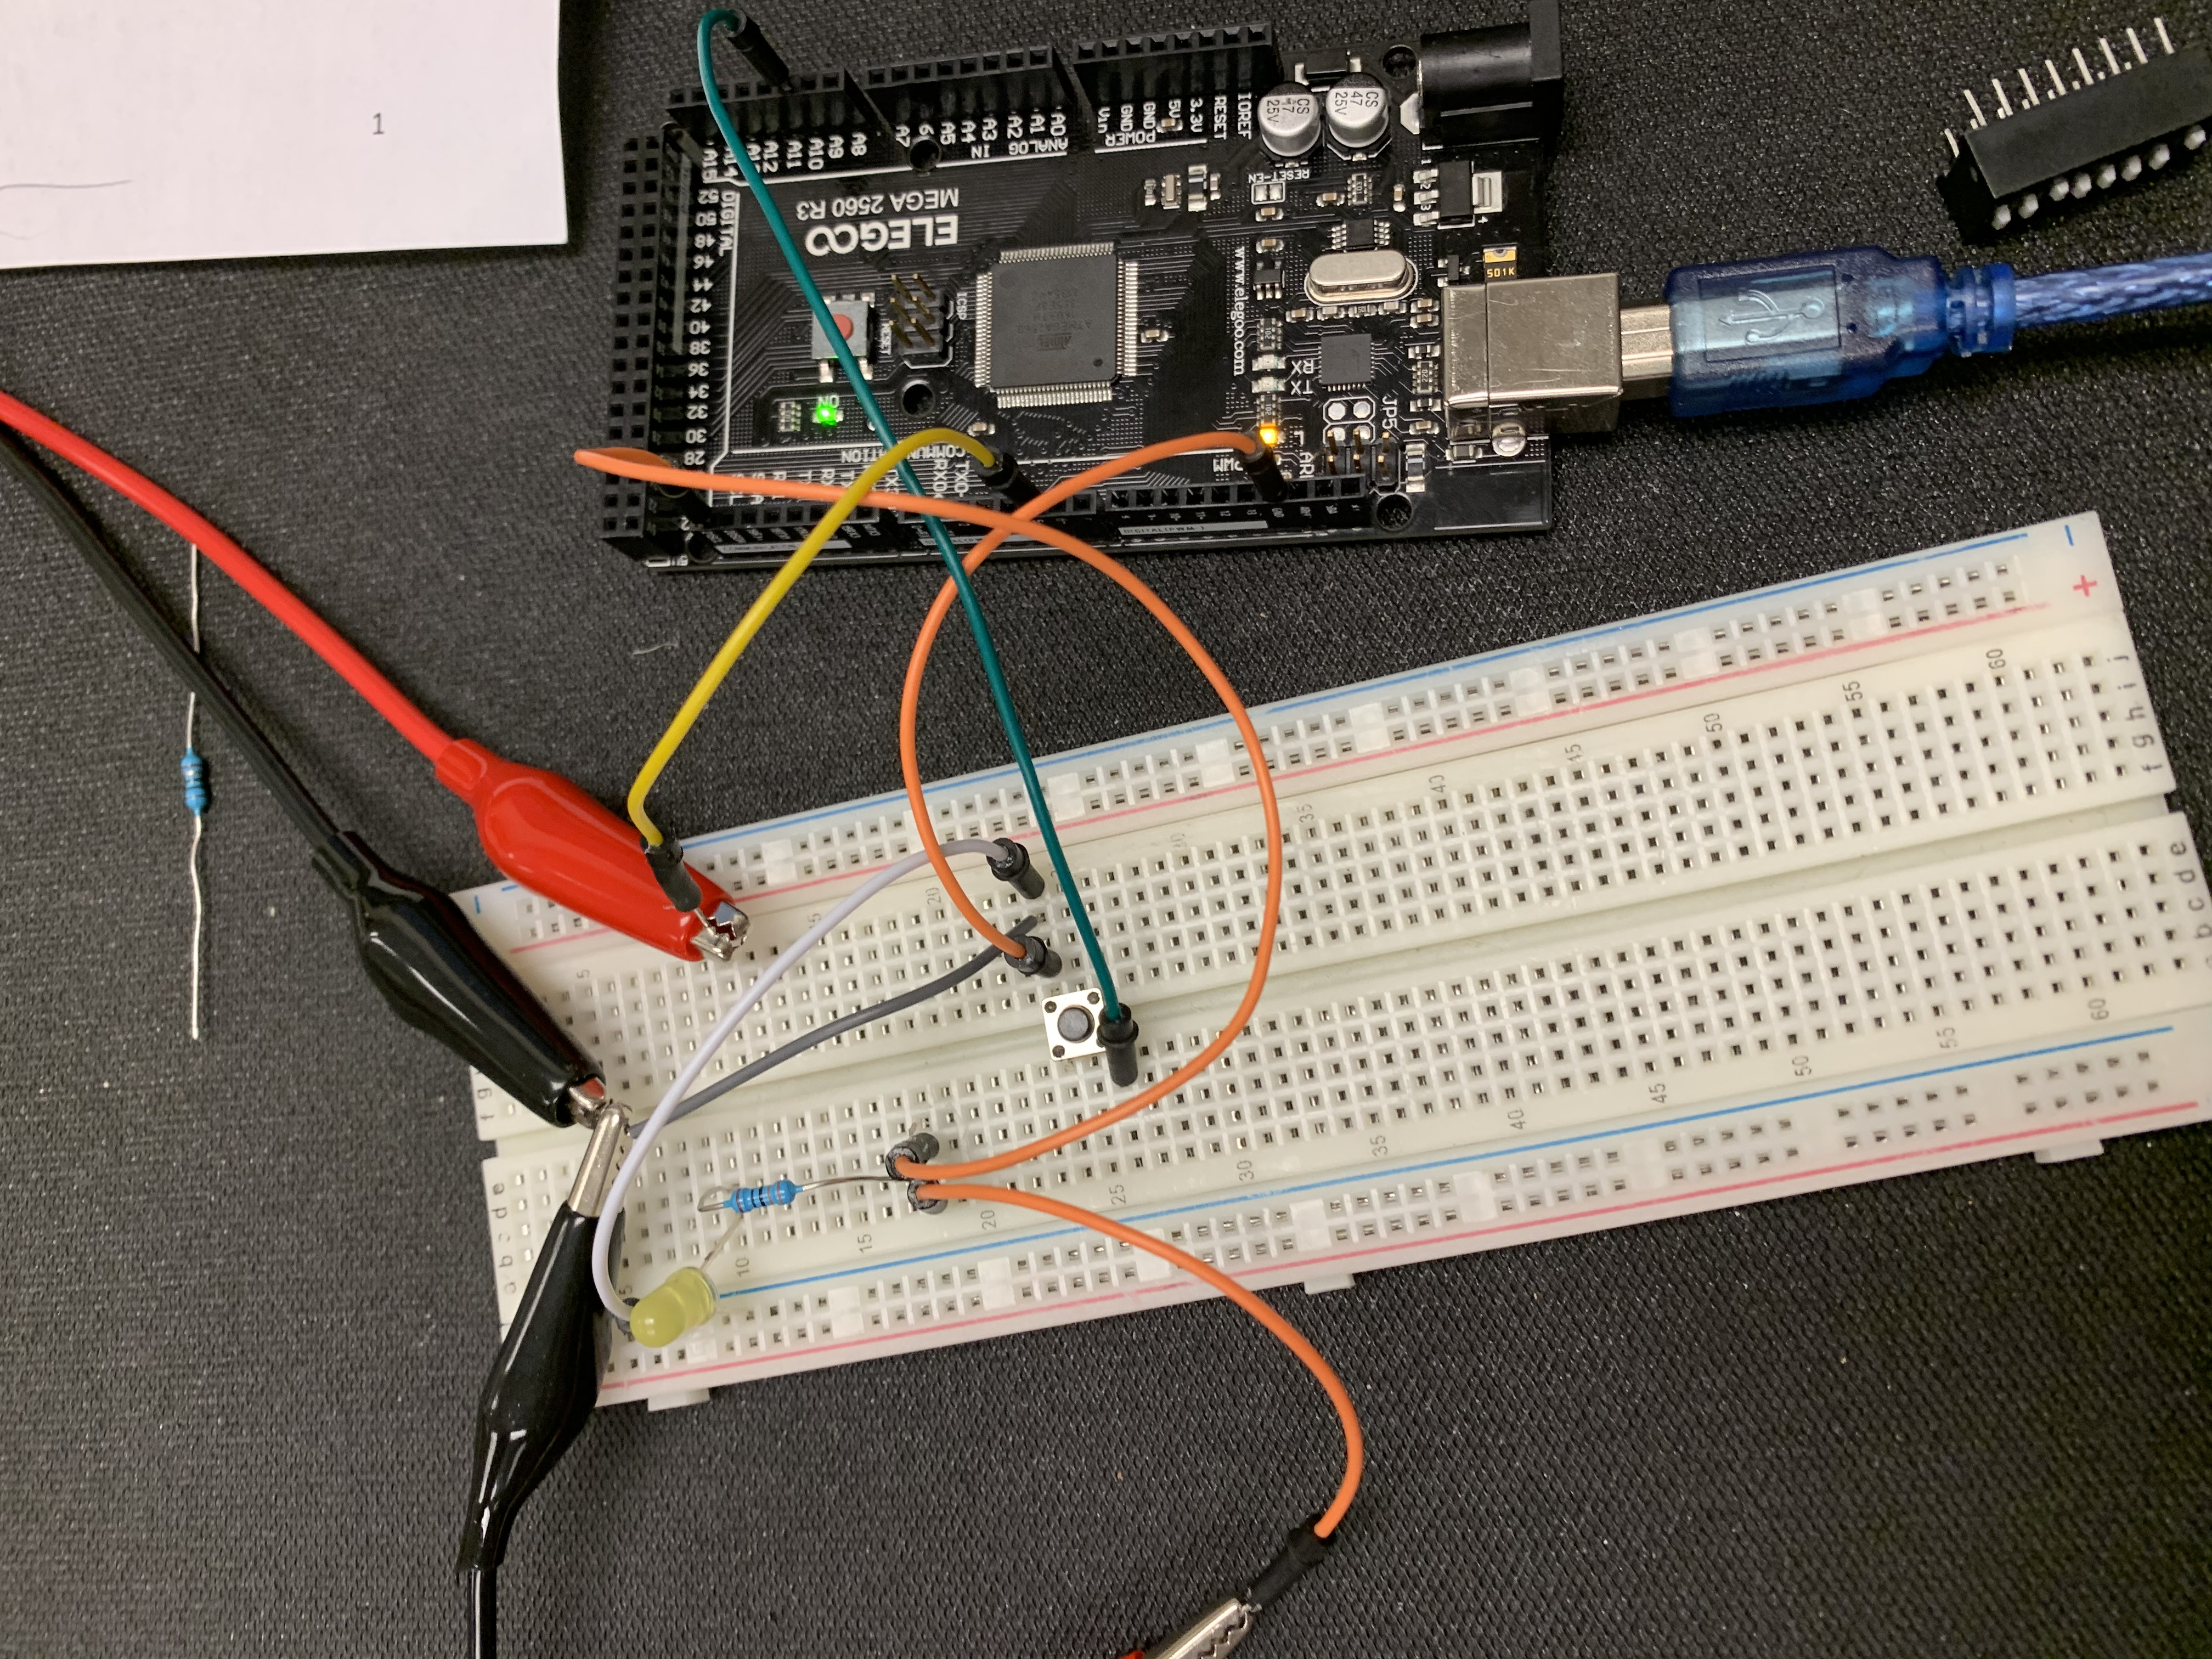
\includegraphics[scale=.1]{images/5-0.jpg}\pagebreak
\begin{enumerate}
	\item Delay is 380ns\\
	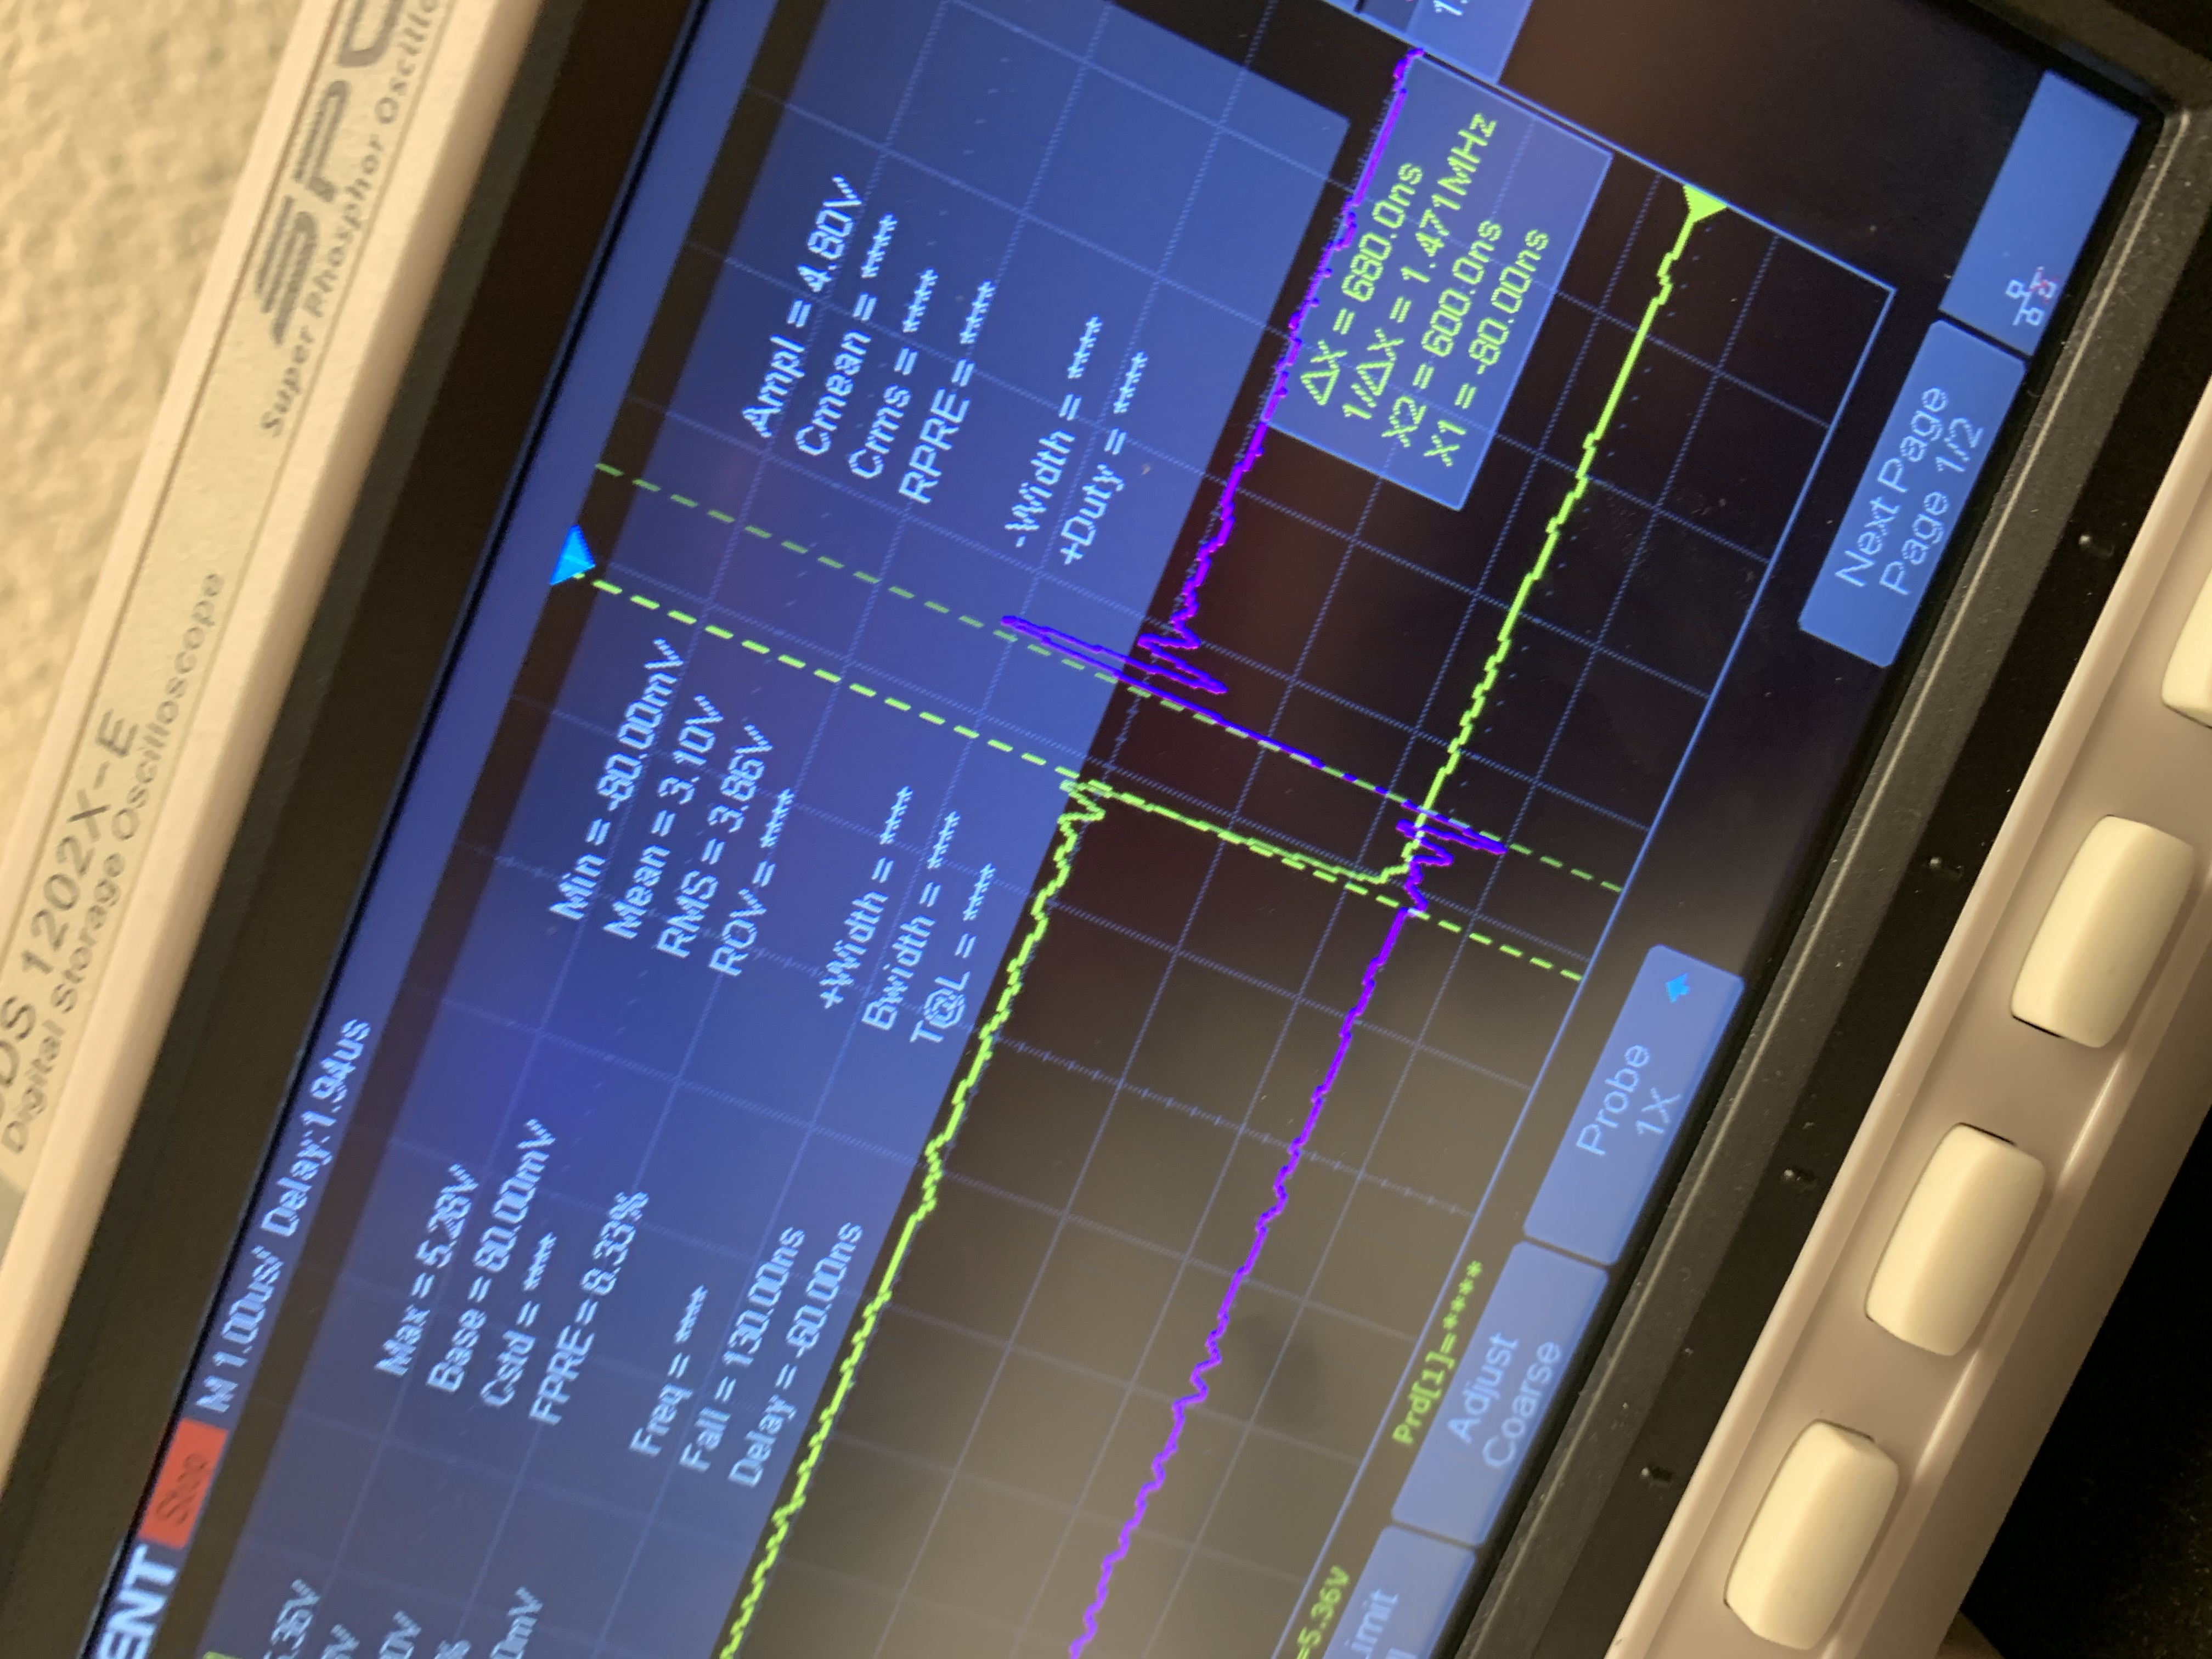
\includegraphics[scale=.1,angle=-90]{images/5-1.jpg}\pagebreak
	\item Delay is 3.140 micro seconds\\
	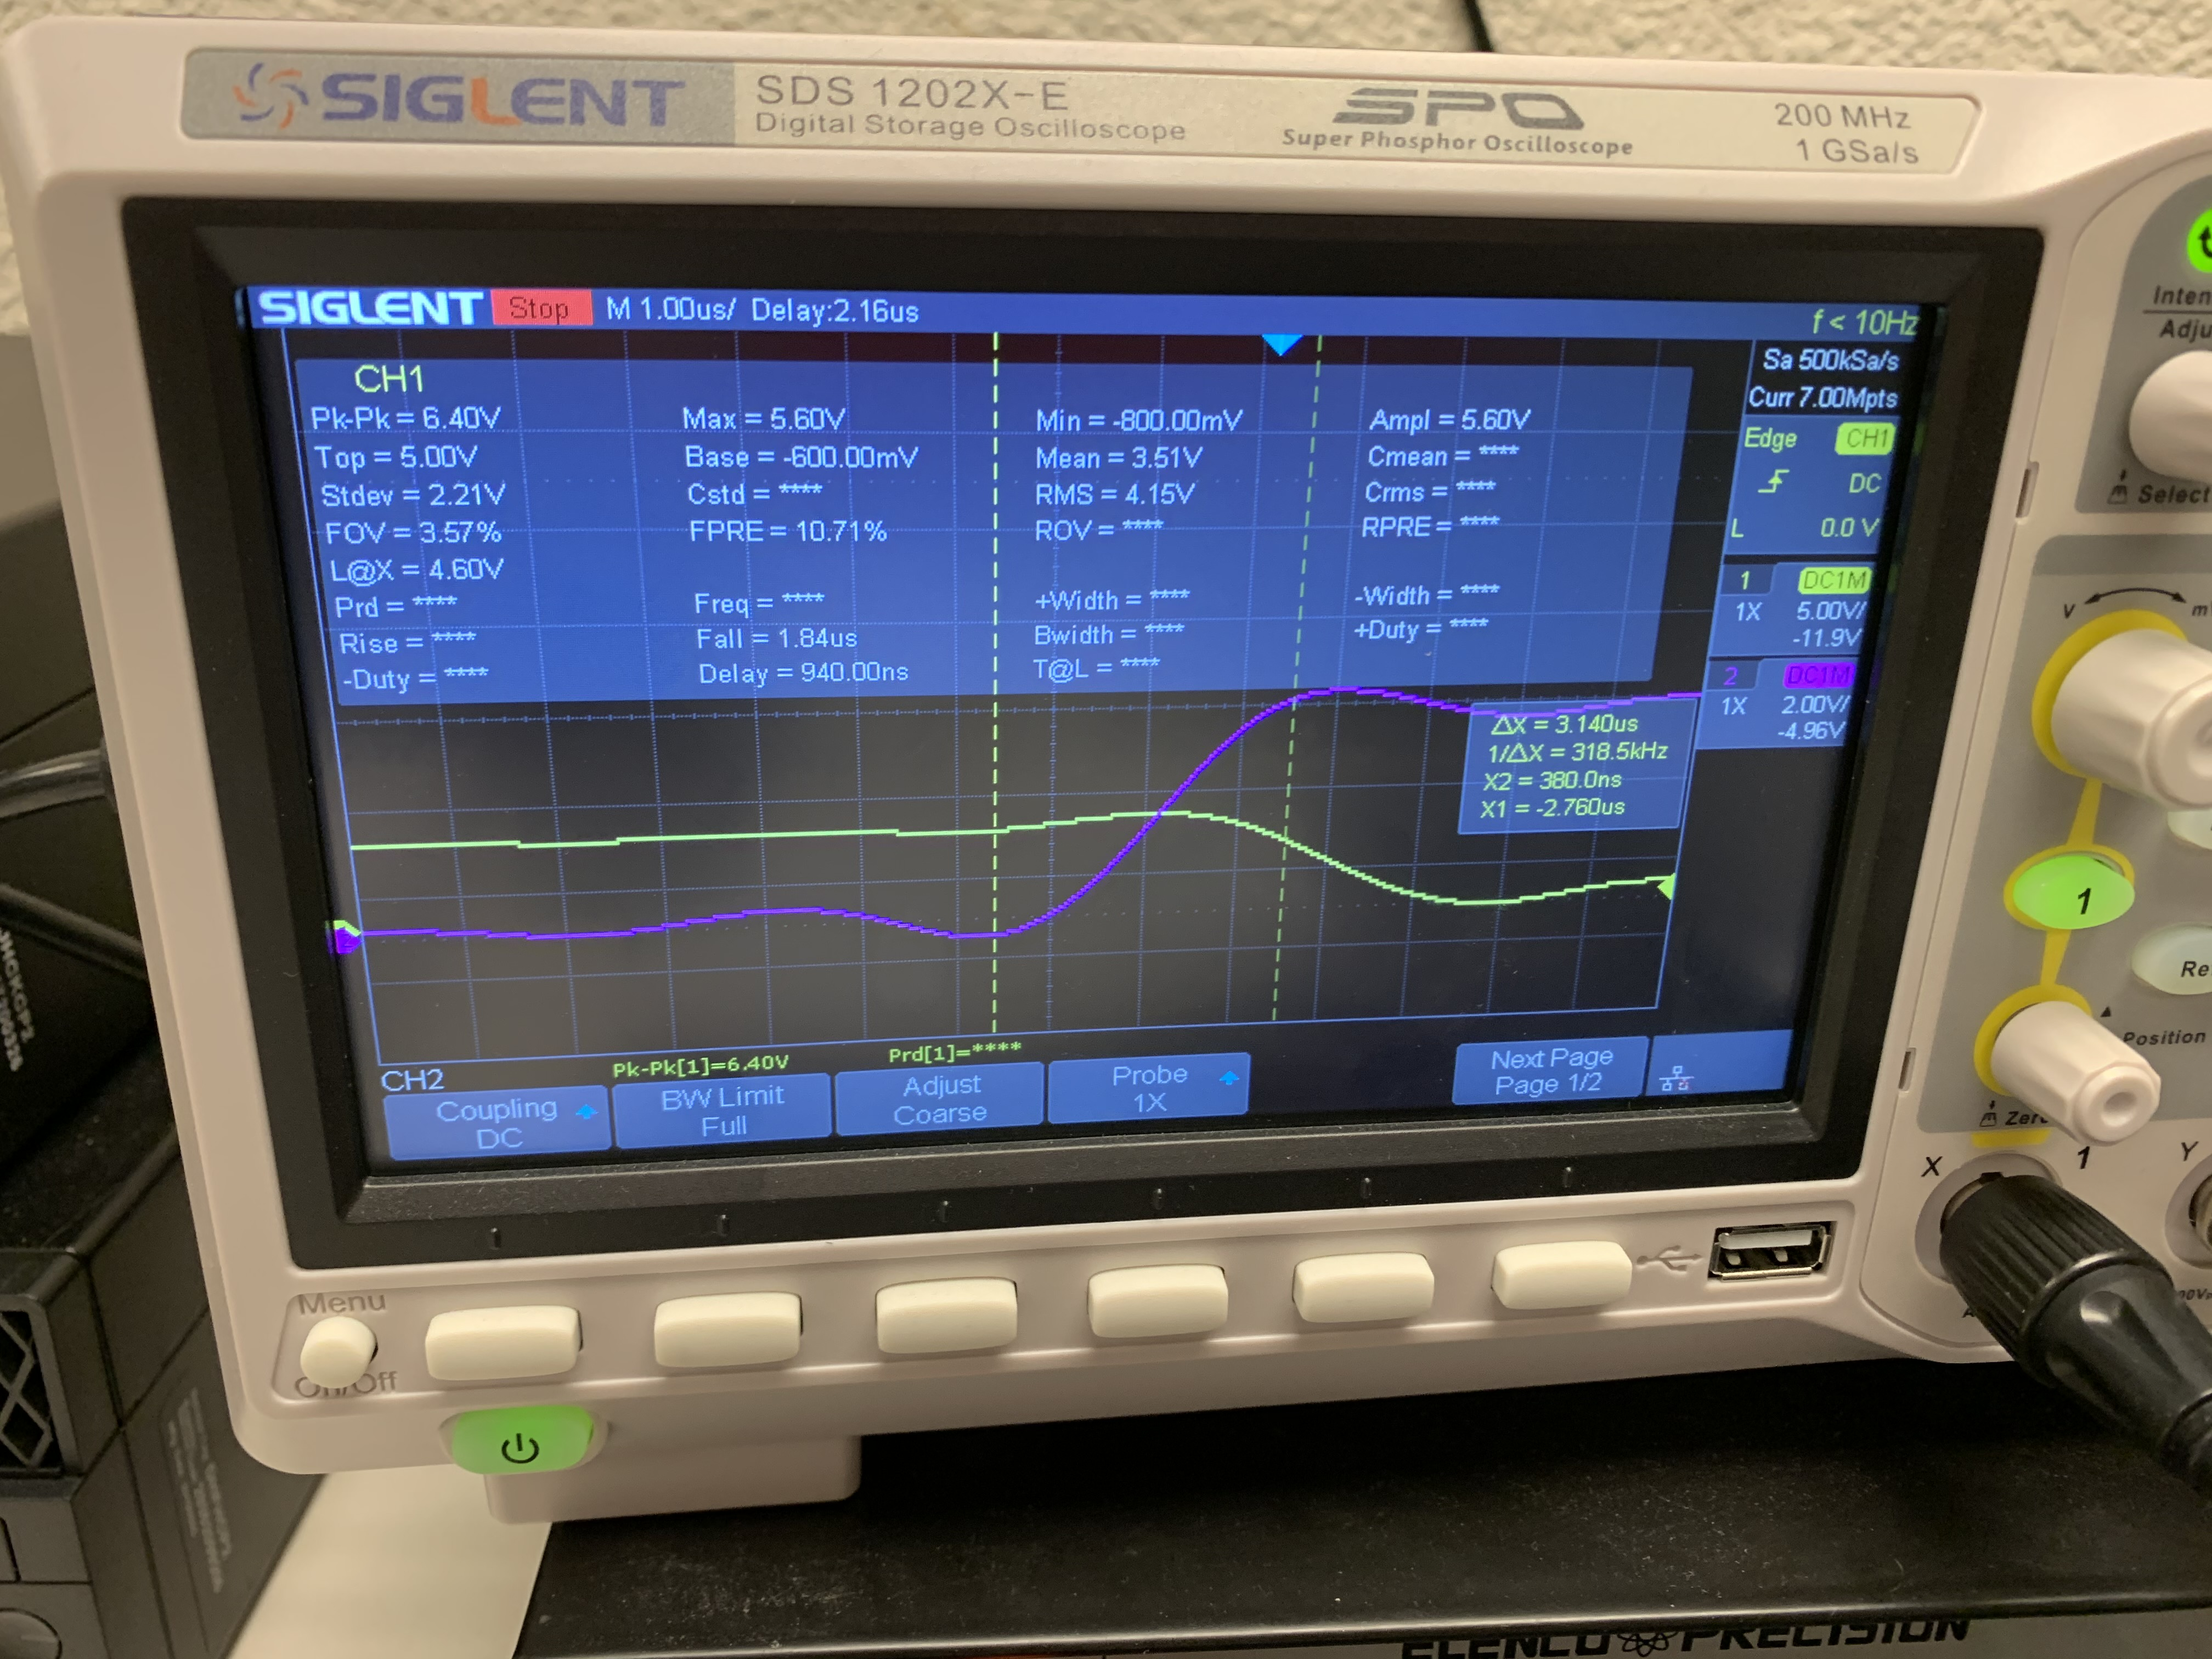
\includegraphics[scale=.1]{images/5-2.jpg}\pagebreak
\end{enumerate}
\lstinputlisting{../sketch/sketch.ino}
\end{document}
